To measure the energy deposits of electromagnetic particles (e.g., electrons, photons) and hadrons (e.g., neutrons, mesons, jets), CMS relies on two calorimeters: the electromagnetic calorimeter and the hadronic calorimeter, both surrounding the CMS tracker and inside the solenoid magnet.

\subsubsection{The Electromagnetic Calorimeter} \label{sec:ECAL}
% Introduce detector, location, basic info (e.g., chamber count)
Immediately surrounding the CMS tracker is the CMS Electromagnetic Calorimeter (ECAL) \cite{ECALTDR}, which allows CMS to measure the energy deposits left by electrons and photons: highly-favored decay modes of the Higgs boson and critical in its discovery. To optimize performance, the ECAL was designed with the following performance goals: excellent energy and spacial resolution, hermeticity and high-granularity, fast particle identification and fast energy and isolation measurements at trigger-level, a wide energy range (\SI{5}{GeV} to \SI{5}{TeV}), and high radiation tolerance. Energy showers from electrons and photons are measured by an array of lead tungstate (PbWO$_4$) scintillating crystals (Fig.~\ref{fig:ECAL}, left). The ECAL is fully hermetic, composed of a barrel (EB) with a pseudorapidity coverage of $|\eta|<1.48$ and two endcaps (EE) that extend the range to $|\eta|<3.0$, (Cutaways of the EE and EB are shown on the right of Fig.~\ref{fig:ECAL}). Within the EB, crystals are grouped into 36 supermodules each containing 1700 crystals, and in each EE crystals are grouped into two dees with 3662 crystals in each, for a total of 75848 crystals in the ECAL. Crystals are oriented in a projective geometry, with an approximately $3^{\circ}$ tilt to avoid aligning crystal gaps with radial particle trajectories. Lining the inner faces of the EE dees in the range $1.65<|\eta|<2.6$ are preshower detectors (ES) made from lead absorbers and silicon strip sensors. A diagram of the ECAL showing the supermodule placement and pseudorapidity coverage is provided on the right of Fig.~\ref{fig:ECALDiagram}.

\begin{figure}[H]
    \centering
    \resizebox{1\textwidth}{!}{
    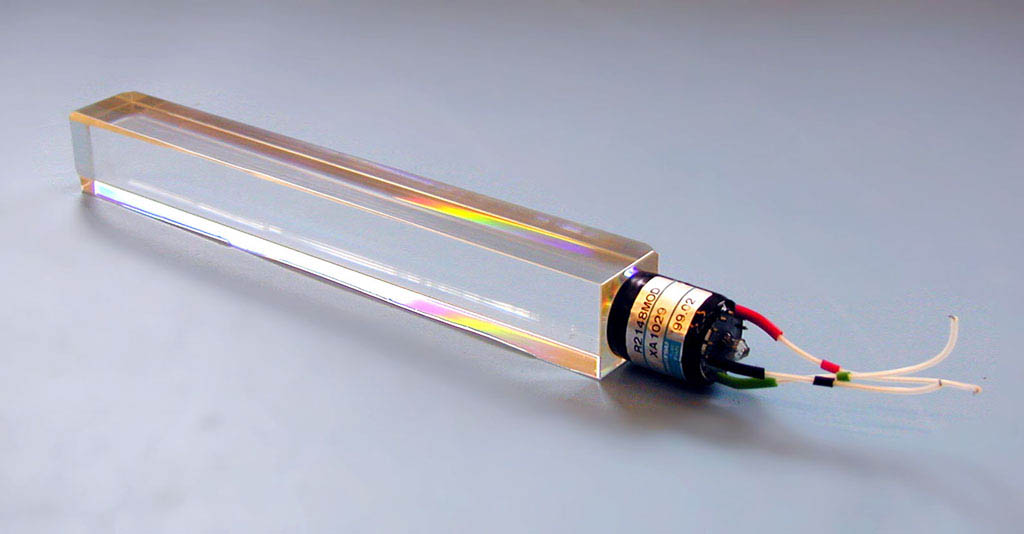
\includegraphics[height=\textwidth]{Images/CMS/ECALCrystal.jpg}
    \quad
    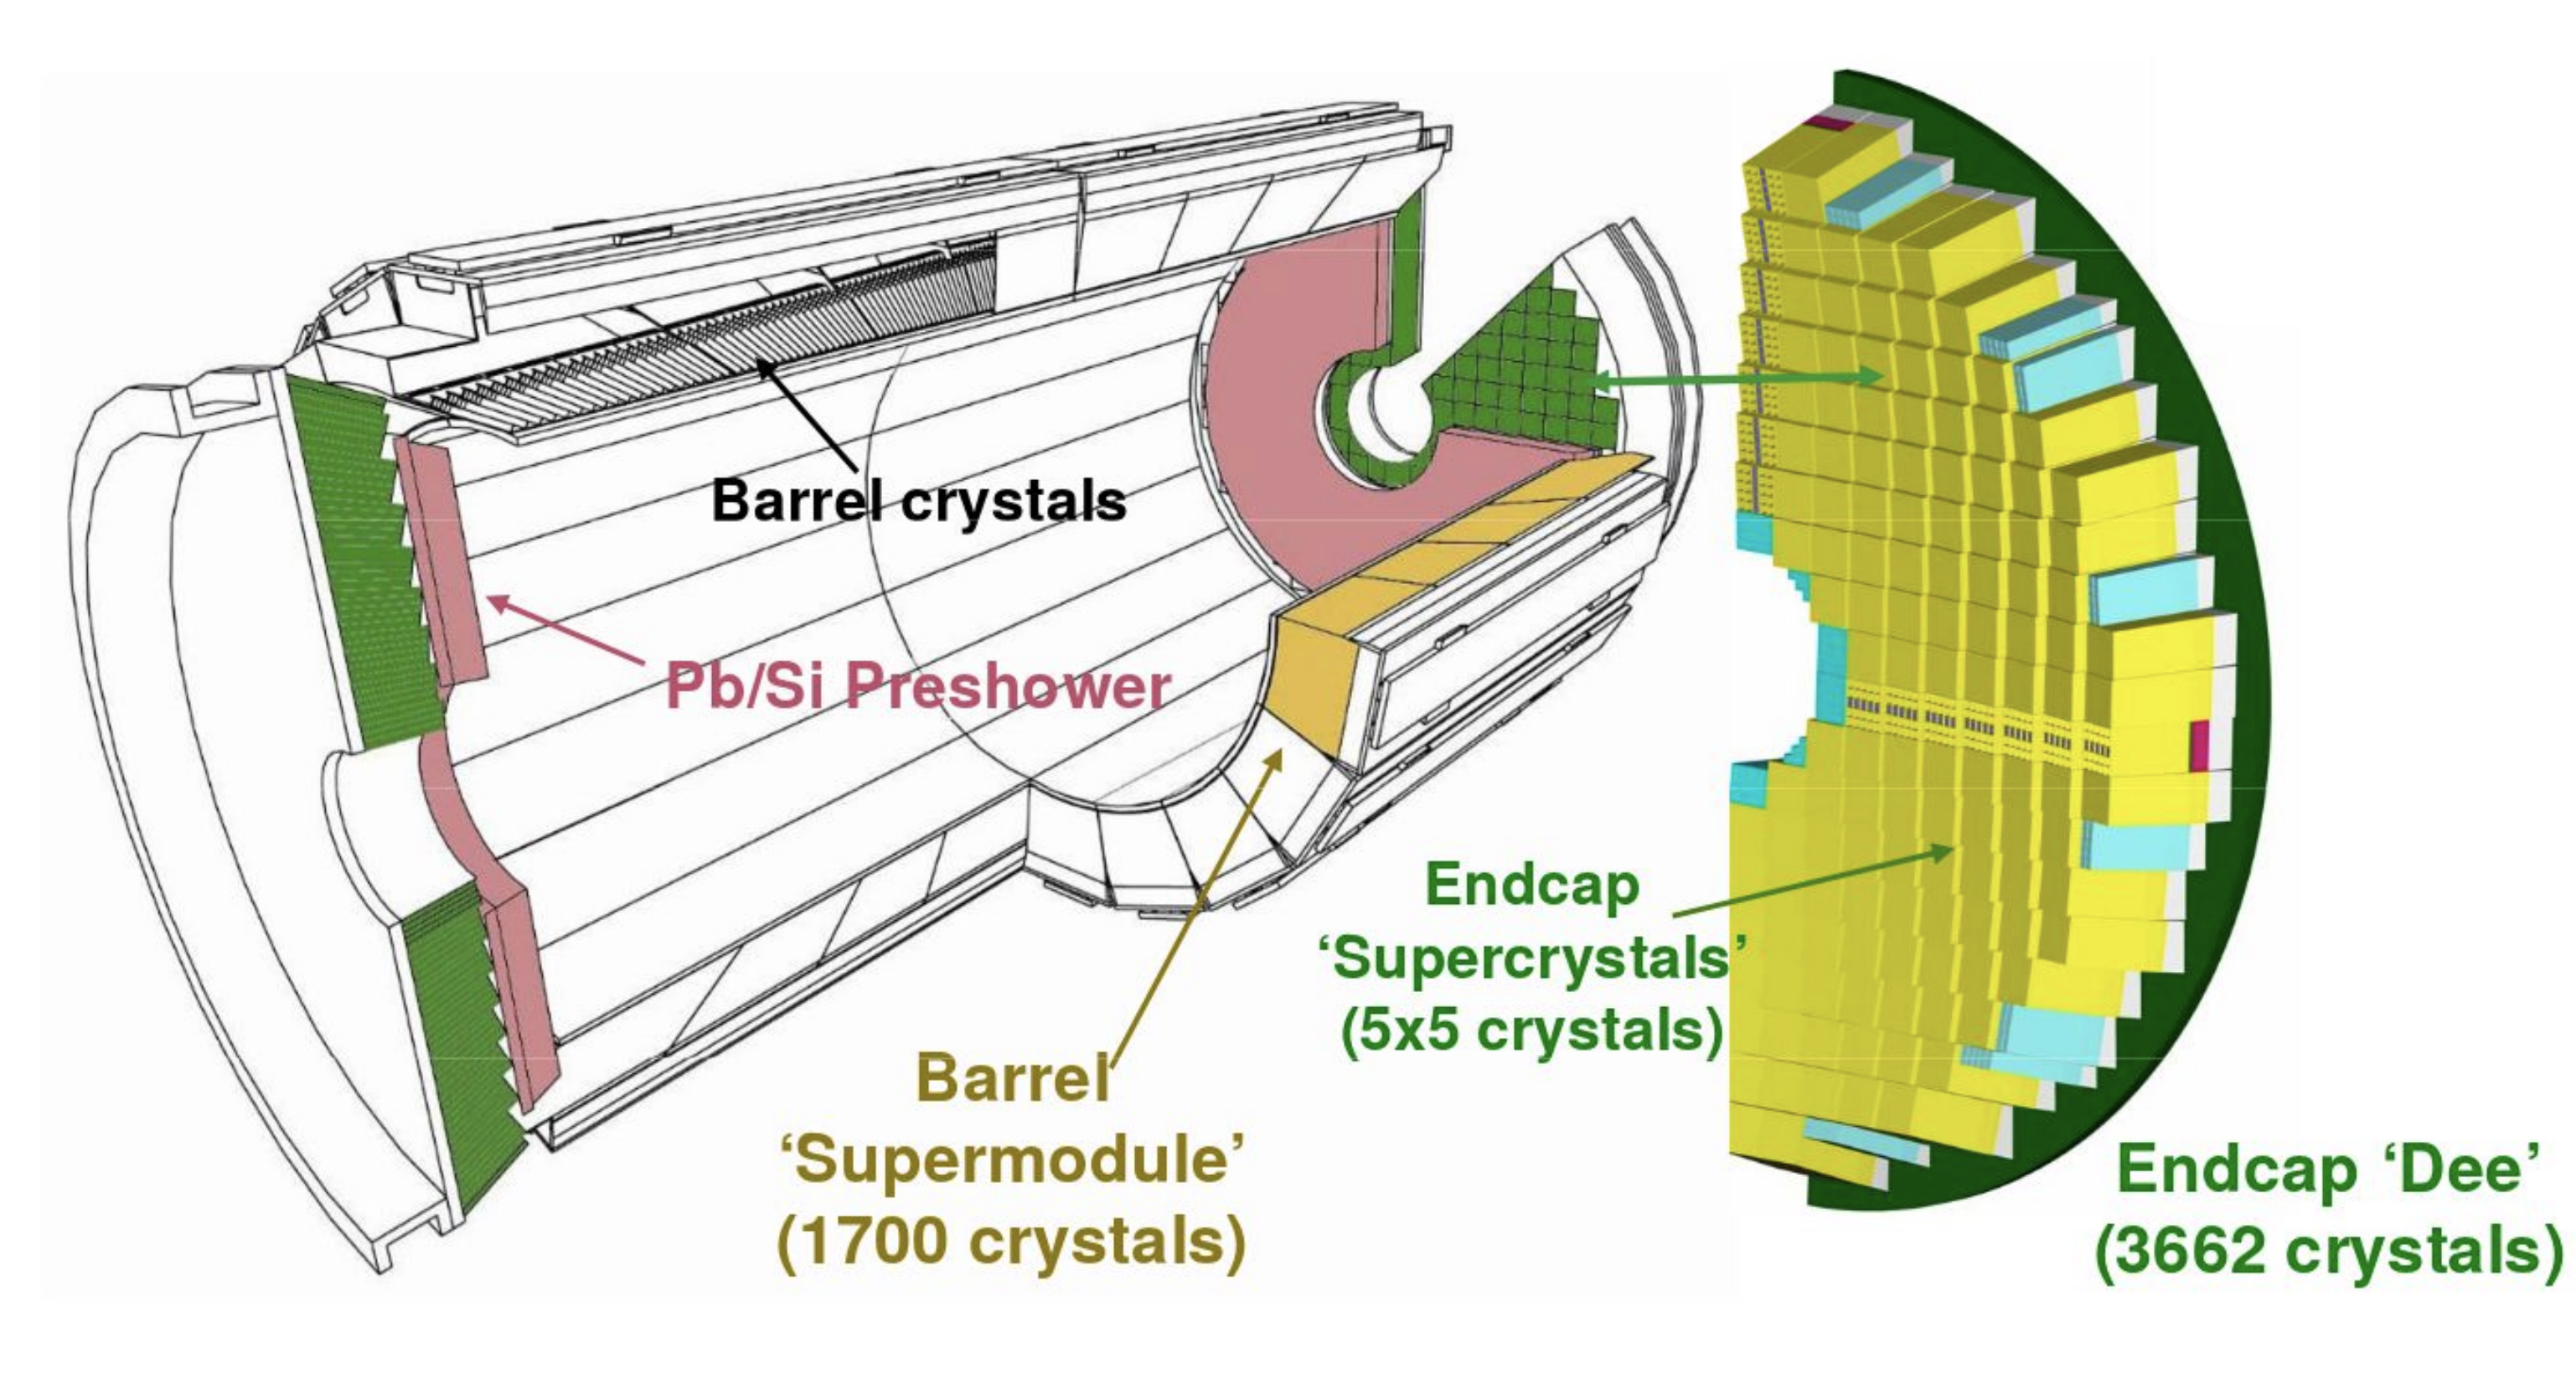
\includegraphics[height=\textwidth]{Images/CMS/ECALDiagram2.png}
    }
    \caption{Left: A photograph of an ECAL crystal. Right: A cutaway showing the orientation of the ECAL supermodules in the barrel and endcap.}
    \label{fig:ECAL}
\end{figure}

\begin{figure}[H]
    \centering
    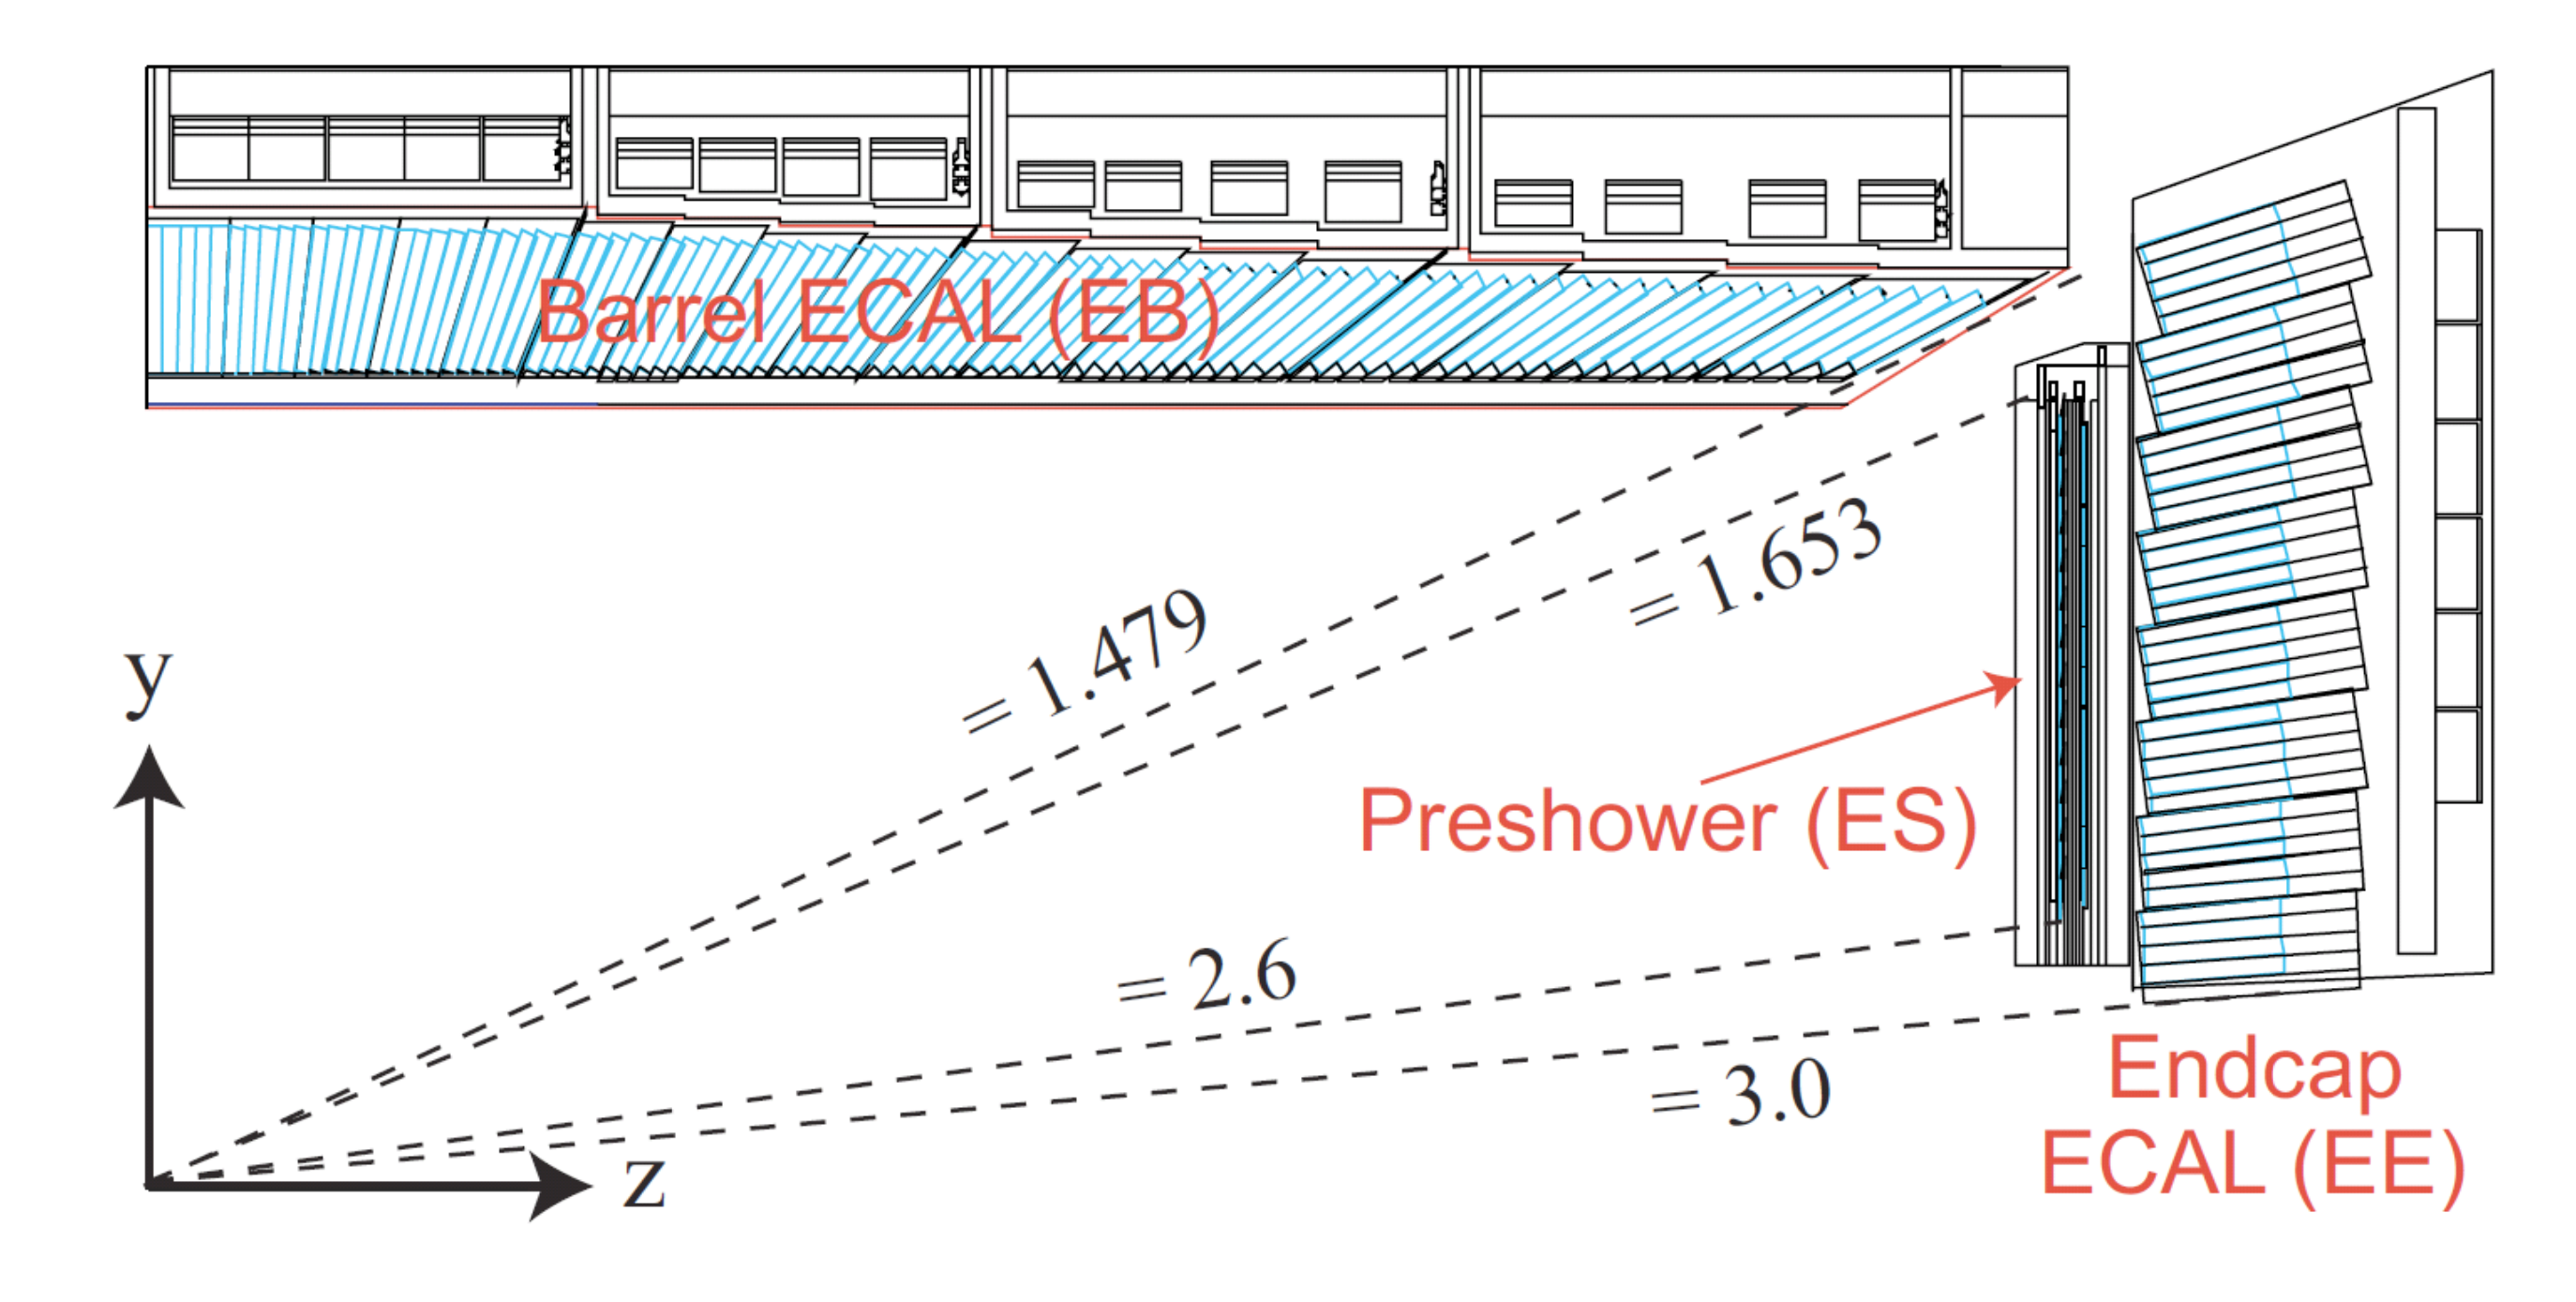
\includegraphics[width=\textwidth]{Images/CMS/ECALDiagram.png}
    \caption{A schematic cutaway showing one quadrant of the ECAL.}
    \label{fig:ECALDiagram}
\end{figure}

\subsubsection{The Hadron Calorimeter} \label{sec:HCAL}
% Introduce detector, location, basic info (e.g., chamber count)
% What is the technology
% Anatomy of a chamber
% How are they arranged in the barrel/endcap
% What do they measure
% Coverage
% Performance

The CMS Hadron Calorimeter (HCAL) \cite{HCALTDR} measures quark, gluon, and neutral particle energy and direction by observing jet energy and missing transverse energy. Within the solenoid magnet, the HCAL is separated into a barrel (HB) and two endcaps (HE), forming the ``central'' HCAL, with a combined pseudorapidity coverage of $|\eta| < 3.0$. An additional two detectors are located outside the solenoid magnet: an array of scintilators that catch the tails of hadronic showers and aid in muon identification called the HCAL Outer calorimeter (HO); and the forward calorimeter (HF), located \SI{6}{m} down the beamline from the ``central'' HCAL (one at each end) and covering the pseudorapidity range $3.0<|\eta|<5.0$, required for accurate missing transverse energy measurements (a diagram showing the arrangement and pseudorapidity coverage of the HCAL and HF is shown in Fig.~\ref{fig:HCALDiagram}). The HB is divided into two half-barrels, each housing 18 wedges ($20^{\circ}$ in $\phi$) of brass alloy absorber plates with a wavelength shifting fiber (WSF) readout. Both HEs are made of The HFs are composed of quartz fibers embedded in a copper absorber matrix. Optical signals are transmitted to hybrid photo diodes (HPD) in the HB and HE, and by photomultiplier tubes (PMT) in the HFs. A photograph of the HB during installation is shown in Fig.~\ref{fig:HCAL}.

\begin{figure}[H]
    \centering
    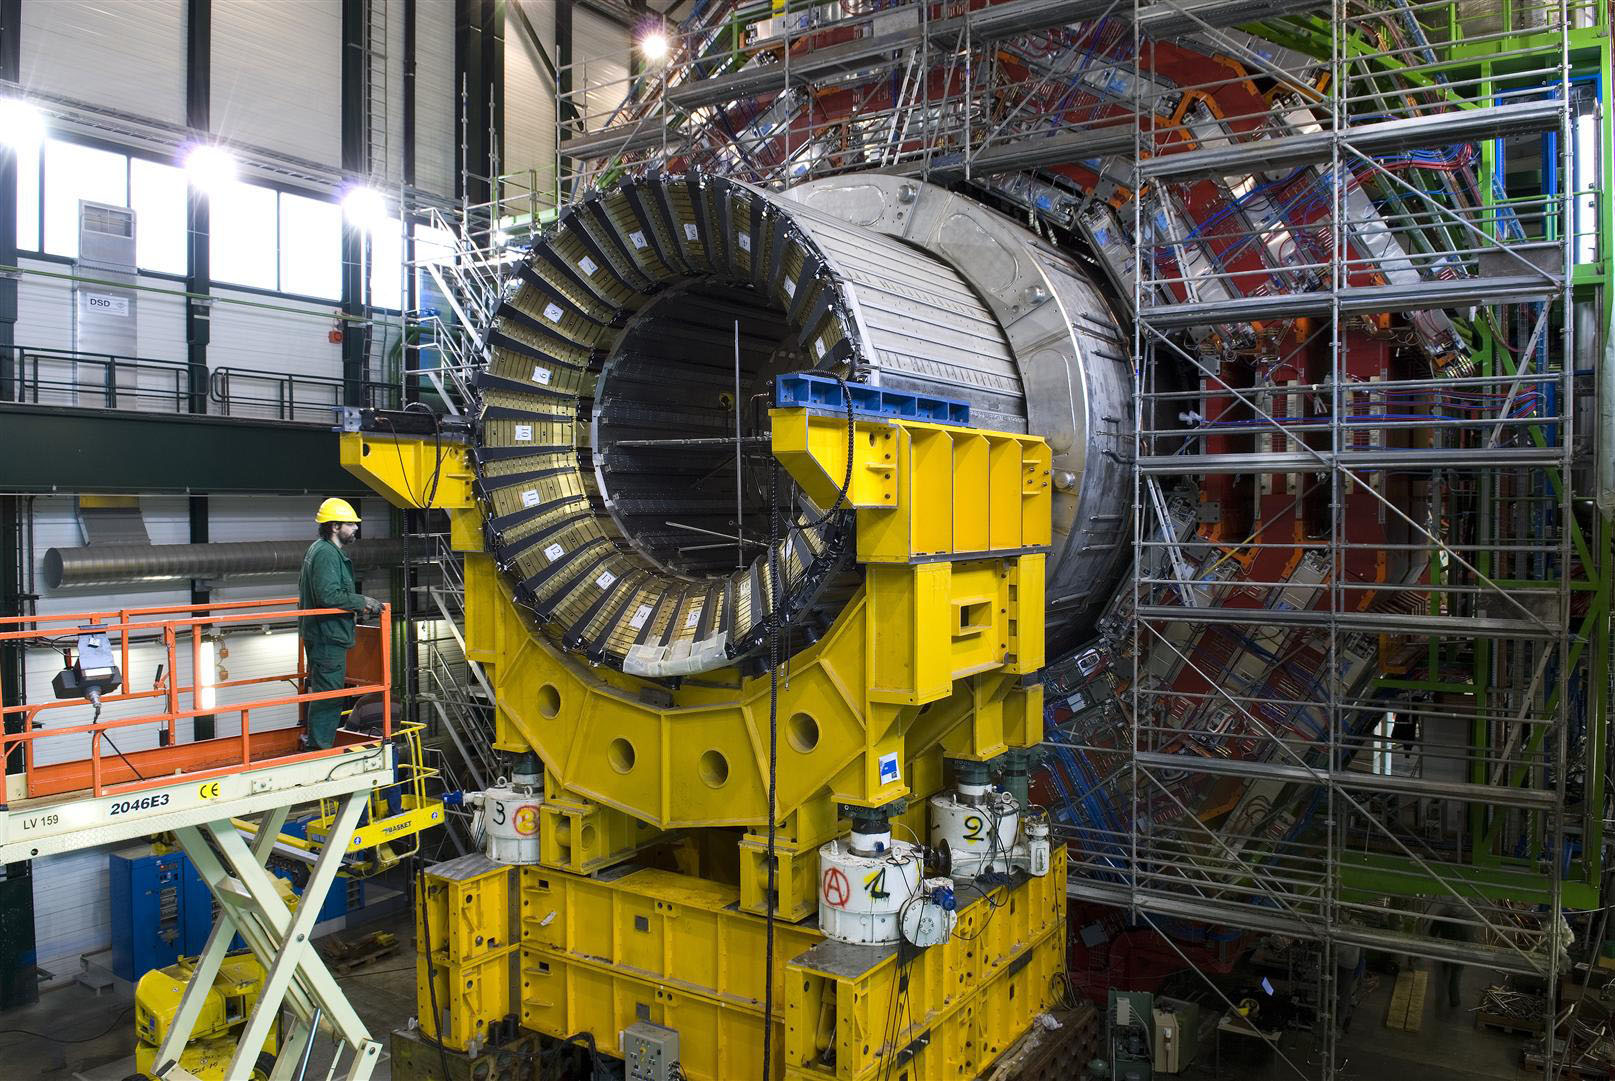
\includegraphics[width=\textwidth]{Images/CMS/HCal.jpg}
    \caption{A photograph showing the HCAL barrel during installation.}
    \label{fig:HCAL}
\end{figure}

\begin{figure}[H]
    \centering
    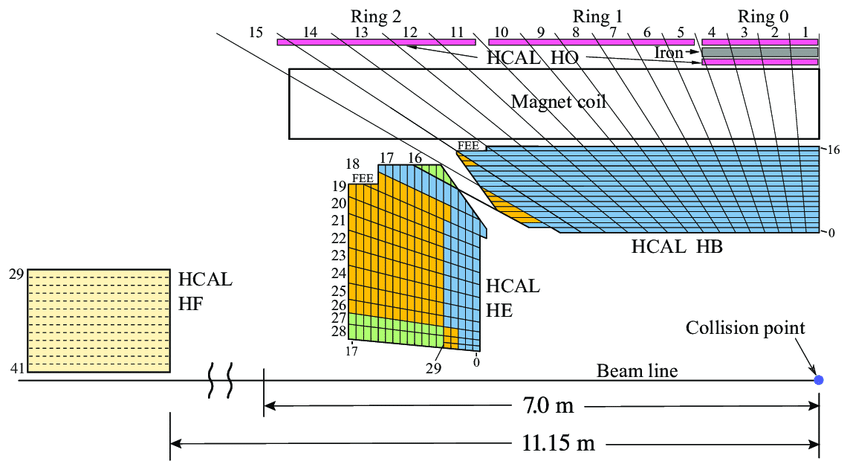
\includegraphics[width=\textwidth]{Images/CMS/HCALDiagram.png}
    \caption{A schematic cutaway showing one quadrant of the HCAL.}
    \label{fig:HCALDiagram}
\end{figure}